\chapter{Objectives}
\label{chap:objetivos_eng}

\drop{N}{owadays}, the largest portion of the information production of documents is carried out using IT tools. Currently, the use of the electronic signature, what guarantees the authenticity of the digital document, is being spread in the public administration, but there is still a large number of people who don't use this procedure. It is very common that in many forms, even being in digital format, documents are presented in a physical medium.

\begin{figure}[h!]
  \begin{center}
      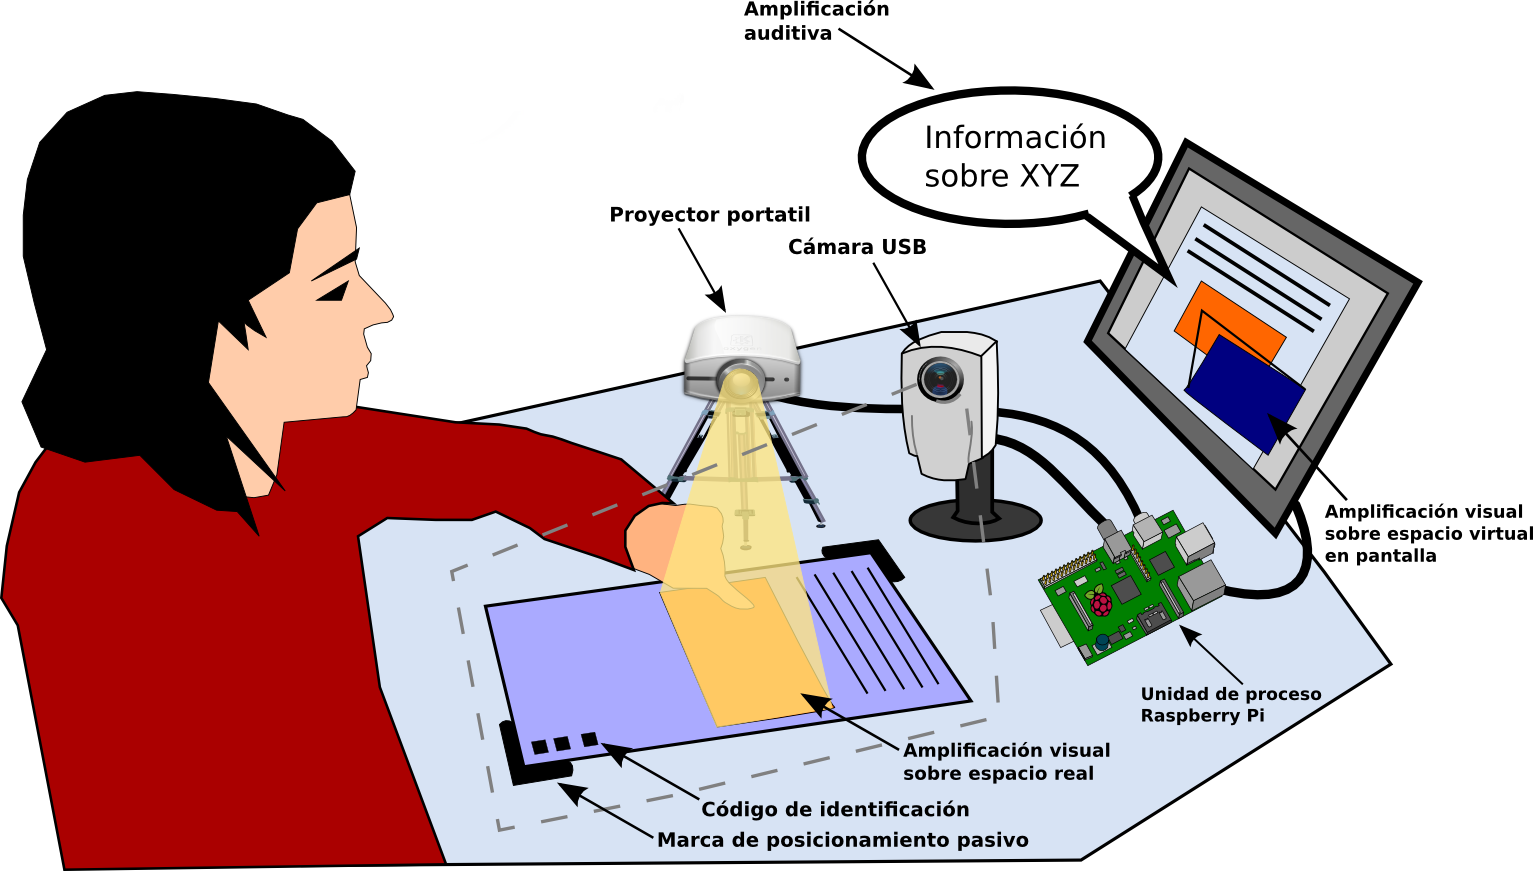
\includegraphics[width=0.85\textwidth]{argos.png}
      \caption{Functional components of \textit{ARgos}}
      \label{fig:diagrama_argos_eng}
    \end{center}
\end{figure}

According to the above, it would be desirable to have a tool that could be able to manage these \textit{«physical»} documents directly. \textit{ARgos} is an INDRA-UCLM Chairs Project that expects the construction of a support system for the management of printed documents using a computer vision system, visual and hearing synthesis and augmented reality techniques. The functional components of the system are shown in the figure \ref{fig:diagrama_argos_eng}.

GrayAR, the proposed end-of-degree project, will discuss the development of the recording, tracking and registration systems and the identification of documents that belong to the \textit{ARgos Project}, whereas the representation part, the delegation of tasks and scripting will be developed by Santiago Sánchez Sobrino in his final year work \textit{«BelfegAR: Platform for the 3D graphic display and delegation of tasks in documental management with augmented reality»}. The specific objectives to be developed are summarised below.


\section{General/Overall objective}
The system uses a low-cost camera as an input in the vision-by-computer module and a portable projection screen to show the visual information, directly aligned with the document of the physical world. It will respond to the requests done by the user in the physical space, expanding information related to the desired action.

The processing unit will take the images taken by the camera as an input and it will generate the output for the projection screen. This output must take into account the relative 3D position between the document and the projection screen to have a perfect register of the visual amplification. The document will be able to move in a specific region of the desktop and the amplification must be perfectly aligned in the physical area. A computer on Raspberry Pi board with ARM architecture will be used. 

\section{Specific objectives}
\begin{itemize}
\item \textbf{Image capture and processing.} We must provide the system with a module to obtain the images and apply a previous process, as it can be the scaling process, thresholding process, edge detection or characteristics detection  \cite{Ortiz} \cite{Bay}. Another task to be done is the calculation of the distortion due to the perspective projection using the extrinsic and intrinsic parameters of the camera. 

\item \textbf{System of document identification.} GrayAR will have a rapid identification system which will use image-retrieval algorithms and it will compare the document which is being analysed with a document database, known for the system. 

\item \textbf{Implementation of tracking and registration techniques.}
The tracking and registration module will have real-time pose calculation features (rotation and translation of the object in the 3D space) and algorithms to estimate and describe the movement, such as \textit{Optical Flow} \cite{LKanade}, all this to get the proper alignment of the displayed information.

\item \textbf{Use of Natural User Interface (NUI) paradigms.}
The user will directly interact with the physical space without using control systems or traditional input devices such as mouse, keyboard, etc. These devices will be replaced by natural functions such as simple gestures of the user’s hands. 

\item \textbf{Facilitation of document management for people with special needs using amplification of the information.} GrayAR will have different ways to amplify the real world information. On the one hand, the visual information will be augmented using a projection screen that will show relevant information directly on the paper space, as well as other additional sources of visual information. 

\item \textbf{It has to be based on low-cost components.} GrayAR must operate with low-cost components to facilitate the deployment at scale, incorporating totally-software correction and 3D registration mechanisms. 

\item \textbf{Multi-platform device (hardware and software).} The GrayAR development will be made following multi-platform free standards, technologies and libraries, with the aim of using it in the largest number of possible platforms, hardware (x86, x86-64 y ARM) as well as software (GNU/Linux, Windows y Mac).
\end{itemize}